% search for all TODOs


\documentclass[11pt]{article}
\usepackage{cs170}


\def\title{Homework 1}
\def\duedate{2025/2/10, at 10:00 pm (grace period until 11:59pm)}

\begin{document}
\maketitle
Due \textbf{\duedate}


\question{Study Group}
List the names and SIDs of the members in your study group.
If you have no collaborators, you must explicitly write ``none''.

\begin{solution} I worked on this homework with the following collaborators:
\begin{itemize}
    \item none,which is only me,Sillycheese
\end{itemize}
\end{solution}

\question{Math Review}

\begin{subparts}
    \item Simplify the following expressions into a single logarithm. Your answer should be in \\
    the form $\log_a{b}$ or $\ln(b)$:
    \begin{enumerate}[(i.)]
        \item $\frac{\ln x}{\ln y}$ \par  
        \begin{solution}
            $log_y{x}$ 
        \end{solution} 
        \item $\ln(x)+\ln(y)$ \par
        \begin{solution}
            $\ln xy$
        \end{solution}
        \item $\ln(x)-\ln(y)$ \par
        \begin{solution}
            $\ln \frac{x}{y}$
        \end{solution}
        \item $170\ln(x)$ \par
        \begin{solution}
            $\ln x^{170}$
        \end{solution}
    \end{enumerate}

    \item Give a simple proof for each of the following identities:
    \begin{enumerate}[(i.)]
        \item $x^{\log_\frac{1}{x}y}= \frac{1}{y}$ \par
        \begin{solution}
            $x^{\log_\frac{1}{x}y}= ((x^{-1})^{-1})^{\log_{x^{-1}}y}=((x^{-1})^{\log_{x^{-1}}y})^{-1}$ \par
            so,we can get $y^{-1}$,and prove it
        \end{solution}
        \item $\sum_{i = 1}^{n}i=\frac{n(n+1)}{2}$ \par
        \begin{solution}
            $\sum_{i = 1}^{n}i=1+2+\dots+n$ \par
            and begin is 1 ,end is n,so we can compute it with that formula, \par
            which is the answer,so prove it.
        \end{solution}
        \item $\sum_{k = 0}^{n}ar^k= 
        \begin{cases}
          a(\frac{1-r^{n+1}}{1-r}),r \neq 1 \\
          a(n+1), r=1
        \end{cases}
        $ \par
        \begin{solution}
            if r=1: \par
            formula=$a(1+1+\dots+1)$,which has $n+1$ numbers \par
            if $r \neq 1$:\par
            formula=$a(1+r+r^{1}+\dots+r^{n})$ \par
            we can get $q$ is r,and begin is$1$,end is$n$
            so use that formula,we can get the answer.
            so prove it.
        \end{solution}
    \end{enumerate}

    \item Consider the following two inequalities: \par
        $$x+3y\leqslant 6$$ 
        $$y\geqslant 2x-5 $$
        Graph out the set of all points (x, y) that satisfy both inequalities above. Clearly mark
your lines and shaded region(s). \\
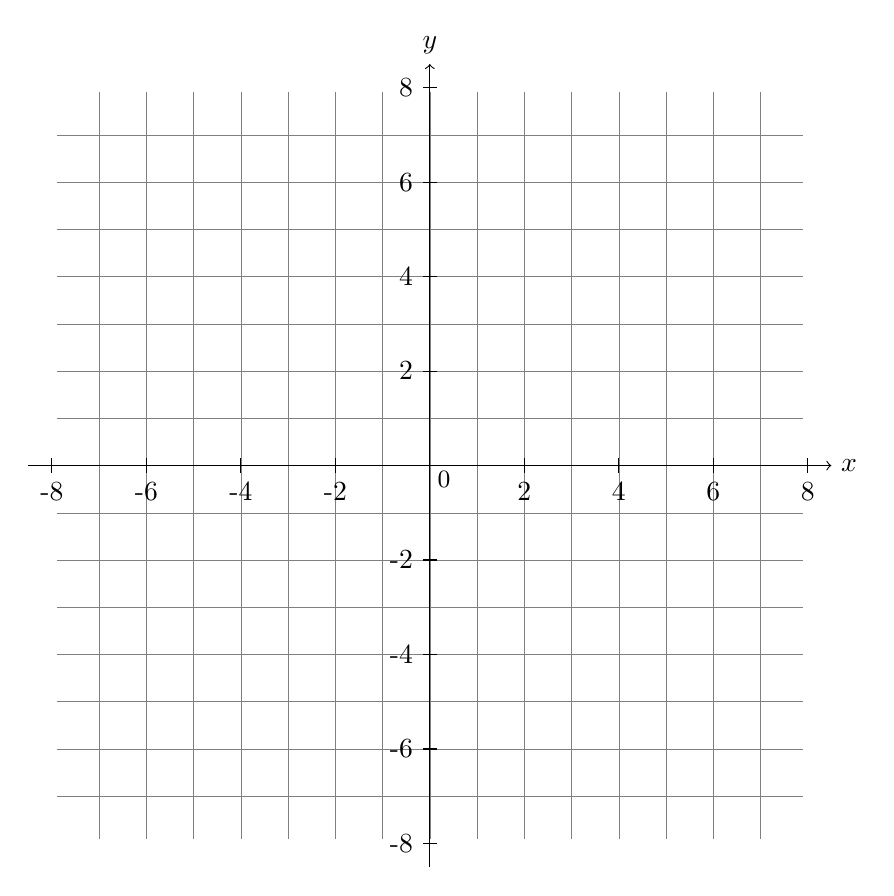
\begin{tikzpicture}[scale=0.6]  
    
    \draw[very thin, gray] (-7.9,-7.9) grid (7.9,7.9);

    
    \draw[->] (-8.5,0) -- (8.5,0) node[right] {$x$}; 
    \draw[->] (0,-8.5) -- (0,8.5) node[above] {$y$}; 

    
    \foreach \x in {-8,-6,-4,-2,2,4,6,8}
        \draw (\x,0.15) -- (\x,-0.15) node[below] {\x};
    \foreach \y in {-8,-6,-4,-2,2,4,6,8}
        \draw (0.15,\y) -- (-0.15,\y) node[left] {\y};

    
    \node at (0.3,-0.3) {\small $0$};
\end{tikzpicture}

\begin{solution} \par
    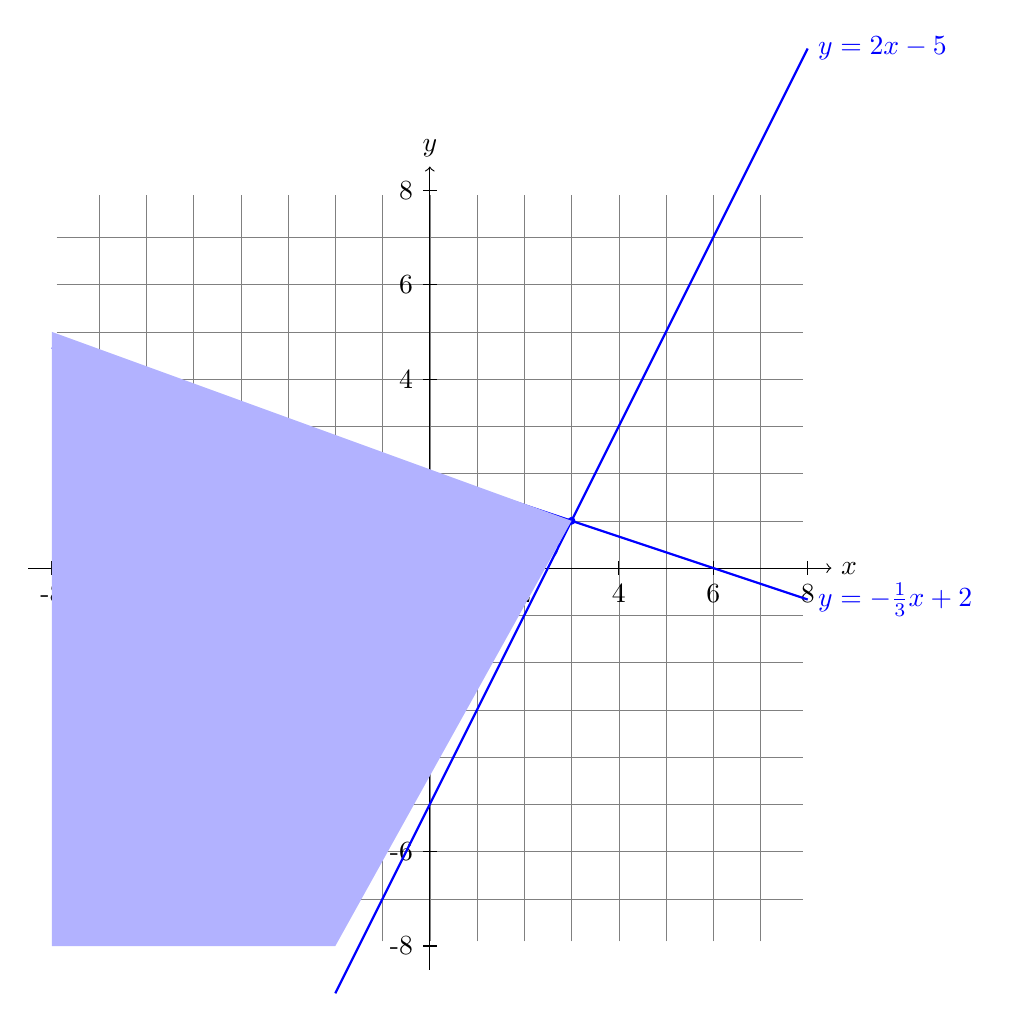
\begin{tikzpicture}[scale=0.6]  
    
        \draw[very thin, gray] (-7.9,-7.9) grid (7.9,7.9);
    
        
        \draw[->] (-8.5,0) -- (8.5,0) node[right] {$x$}; 
        \draw[->] (0,-8.5) -- (0,8.5) node[above] {$y$}; 
    
        
        \foreach \x in {-8,-6,-4,-2,2,4,6,8}
            \draw (\x,0.15) -- (\x,-0.15) node[below] {\x};
        \foreach \y in {-8,-6,-4,-2,2,4,6,8}
            \draw (0.15,\y) -- (-0.15,\y) node[left] {\y};
    
        
        \node at (0.3,-0.3) {\small $0$};

        % funcs
        \draw[thick, blue, domain=-8:8, samples=100] plot (\x, {2-1/3*(\x)}) 
        node[right] {$y = -\frac{1}{3}x + 2$};

        \draw[thick, blue, domain=-2:8, samples=100] plot (\x, {-5+2*(\x)}) 
        node[right] {$y = 2x-5$};

        % inter
        \filldraw[blue] (3,1) circle (2pt) node[below left] {$(3,1)$};

        \fill[blue!30] (-8,5) -- (3,1) -- (-2,-8) -- (-8,-8) -- cycle;

    \end{tikzpicture}
\end{solution}
    
\end{subparts}

\question{Asymptotics Practice}

\begin{subparts}
    \item For each pair of functions f and g below, specify whether f = O(g), g = O(f ), or both.
    No justification needed.\par
    \begin{solution}
        \begin{enumerate}[i.]
            \item both
            \item both
            \item $f=O(g)$
            \item $f=O(g)$
            \item $f=O(g)$
            \item $f=O(g)$
        \end{enumerate}
    \end{solution}

    \item Consider the two functions f (n) = 1 + b + b2 + ···+ bn and g(n) = bn for an arbitrary
    constant b > 0. Similar to what you did in the previous part, specify whether f =
    O(g), g = O(f ), or both. Justify your answer.
    Hint: the asymptotic relationship between f and g varies depending on the specific value
    of b.
    This content is protected and may not be shared, uploaded, or distributed.
    
    \begin{solution} \par
        $g = O(f)$ for all b > 0, as $g(n) ≤ f(n)$ for all n. \par
        only if $b>1$ , $f=O(g)$

    \end{solution}
\end{subparts}

\question{Recurrence Relations}

For each part, find the asymptotic order of growth of $T (n)$; that is, find a function g such that
$T (n) = Θ(g(n))$. Show your reasoning and do not directly apply the Master Theorem;
doing so will yield 0 credit. \par
In all subparts, you may ignore any issues arising from whether a number is an integer.

\begin{enumerate}
    \item $T (n) = 2T (n/3) + 5n$ \par
    \begin{solution}
        $\sum_{k = 0}^{\log_3{n}}(\frac{2}{3})^k\cdot5n  $ \par
        then it is $\varTheta (n)$
    \end{solution}
    \item An algorithm A takes Θ(n log n) time to partition the input into 5 sub-problems of
    size n/5 each and then recursively runs itself on 3 of those subproblems. Describe the
    recurrence relation for the run-time T (n) of A and find its asymptotic order of growth. \par
    \begin{solution}
        this is $\varTheta (n\log{n})$
    \end{solution}
    \item $T (n) = T (3n/5) + T (4n/5) (We have T (1) = 1)$ \par
    \begin{solution}
        this is $\varTheta (n^2)$
    \end{solution}
    \item $T(n)=T(\sqrt{n})+1$ \par
    \begin{solution}
        this is $\varTheta (log{log{n}})$
    \end{solution}
\end{enumerate}

\end{document}
